\documentclass[]{article}
\usepackage{lmodern}
\usepackage{amssymb,amsmath}
\usepackage{ifxetex,ifluatex}
\usepackage{fixltx2e} % provides \textsubscript
\ifnum 0\ifxetex 1\fi\ifluatex 1\fi=0 % if pdftex
  \usepackage[T1]{fontenc}
  \usepackage[utf8]{inputenc}
\else % if luatex or xelatex
  \ifxetex
    \usepackage{mathspec}
  \else
    \usepackage{fontspec}
  \fi
  \defaultfontfeatures{Ligatures=TeX,Scale=MatchLowercase}
\fi
% use upquote if available, for straight quotes in verbatim environments
\IfFileExists{upquote.sty}{\usepackage{upquote}}{}
% use microtype if available
\IfFileExists{microtype.sty}{%
\usepackage{microtype}
\UseMicrotypeSet[protrusion]{basicmath} % disable protrusion for tt fonts
}{}
\usepackage[margin=1in]{geometry}
\usepackage{hyperref}
\hypersetup{unicode=true,
            pdfborder={0 0 0},
            breaklinks=true}
\urlstyle{same}  % don't use monospace font for urls
\usepackage{color}
\usepackage{fancyvrb}
\newcommand{\VerbBar}{|}
\newcommand{\VERB}{\Verb[commandchars=\\\{\}]}
\DefineVerbatimEnvironment{Highlighting}{Verbatim}{commandchars=\\\{\}}
% Add ',fontsize=\small' for more characters per line
\usepackage{framed}
\definecolor{shadecolor}{RGB}{248,248,248}
\newenvironment{Shaded}{\begin{snugshade}}{\end{snugshade}}
\newcommand{\AlertTok}[1]{\textcolor[rgb]{0.94,0.16,0.16}{#1}}
\newcommand{\AnnotationTok}[1]{\textcolor[rgb]{0.56,0.35,0.01}{\textbf{\textit{#1}}}}
\newcommand{\AttributeTok}[1]{\textcolor[rgb]{0.77,0.63,0.00}{#1}}
\newcommand{\BaseNTok}[1]{\textcolor[rgb]{0.00,0.00,0.81}{#1}}
\newcommand{\BuiltInTok}[1]{#1}
\newcommand{\CharTok}[1]{\textcolor[rgb]{0.31,0.60,0.02}{#1}}
\newcommand{\CommentTok}[1]{\textcolor[rgb]{0.56,0.35,0.01}{\textit{#1}}}
\newcommand{\CommentVarTok}[1]{\textcolor[rgb]{0.56,0.35,0.01}{\textbf{\textit{#1}}}}
\newcommand{\ConstantTok}[1]{\textcolor[rgb]{0.00,0.00,0.00}{#1}}
\newcommand{\ControlFlowTok}[1]{\textcolor[rgb]{0.13,0.29,0.53}{\textbf{#1}}}
\newcommand{\DataTypeTok}[1]{\textcolor[rgb]{0.13,0.29,0.53}{#1}}
\newcommand{\DecValTok}[1]{\textcolor[rgb]{0.00,0.00,0.81}{#1}}
\newcommand{\DocumentationTok}[1]{\textcolor[rgb]{0.56,0.35,0.01}{\textbf{\textit{#1}}}}
\newcommand{\ErrorTok}[1]{\textcolor[rgb]{0.64,0.00,0.00}{\textbf{#1}}}
\newcommand{\ExtensionTok}[1]{#1}
\newcommand{\FloatTok}[1]{\textcolor[rgb]{0.00,0.00,0.81}{#1}}
\newcommand{\FunctionTok}[1]{\textcolor[rgb]{0.00,0.00,0.00}{#1}}
\newcommand{\ImportTok}[1]{#1}
\newcommand{\InformationTok}[1]{\textcolor[rgb]{0.56,0.35,0.01}{\textbf{\textit{#1}}}}
\newcommand{\KeywordTok}[1]{\textcolor[rgb]{0.13,0.29,0.53}{\textbf{#1}}}
\newcommand{\NormalTok}[1]{#1}
\newcommand{\OperatorTok}[1]{\textcolor[rgb]{0.81,0.36,0.00}{\textbf{#1}}}
\newcommand{\OtherTok}[1]{\textcolor[rgb]{0.56,0.35,0.01}{#1}}
\newcommand{\PreprocessorTok}[1]{\textcolor[rgb]{0.56,0.35,0.01}{\textit{#1}}}
\newcommand{\RegionMarkerTok}[1]{#1}
\newcommand{\SpecialCharTok}[1]{\textcolor[rgb]{0.00,0.00,0.00}{#1}}
\newcommand{\SpecialStringTok}[1]{\textcolor[rgb]{0.31,0.60,0.02}{#1}}
\newcommand{\StringTok}[1]{\textcolor[rgb]{0.31,0.60,0.02}{#1}}
\newcommand{\VariableTok}[1]{\textcolor[rgb]{0.00,0.00,0.00}{#1}}
\newcommand{\VerbatimStringTok}[1]{\textcolor[rgb]{0.31,0.60,0.02}{#1}}
\newcommand{\WarningTok}[1]{\textcolor[rgb]{0.56,0.35,0.01}{\textbf{\textit{#1}}}}
\usepackage{graphicx,grffile}
\makeatletter
\def\maxwidth{\ifdim\Gin@nat@width>\linewidth\linewidth\else\Gin@nat@width\fi}
\def\maxheight{\ifdim\Gin@nat@height>\textheight\textheight\else\Gin@nat@height\fi}
\makeatother
% Scale images if necessary, so that they will not overflow the page
% margins by default, and it is still possible to overwrite the defaults
% using explicit options in \includegraphics[width, height, ...]{}
\setkeys{Gin}{width=\maxwidth,height=\maxheight,keepaspectratio}
\IfFileExists{parskip.sty}{%
\usepackage{parskip}
}{% else
\setlength{\parindent}{0pt}
\setlength{\parskip}{6pt plus 2pt minus 1pt}
}
\setlength{\emergencystretch}{3em}  % prevent overfull lines
\providecommand{\tightlist}{%
  \setlength{\itemsep}{0pt}\setlength{\parskip}{0pt}}
\setcounter{secnumdepth}{0}
% Redefines (sub)paragraphs to behave more like sections
\ifx\paragraph\undefined\else
\let\oldparagraph\paragraph
\renewcommand{\paragraph}[1]{\oldparagraph{#1}\mbox{}}
\fi
\ifx\subparagraph\undefined\else
\let\oldsubparagraph\subparagraph
\renewcommand{\subparagraph}[1]{\oldsubparagraph{#1}\mbox{}}
\fi

%%% Use protect on footnotes to avoid problems with footnotes in titles
\let\rmarkdownfootnote\footnote%
\def\footnote{\protect\rmarkdownfootnote}

%%% Change title format to be more compact
\usepackage{titling}

% Create subtitle command for use in maketitle
\providecommand{\subtitle}[1]{
  \posttitle{
    \begin{center}\large#1\end{center}
    }
}

\setlength{\droptitle}{-2em}

  \title{}
    \pretitle{\vspace{\droptitle}}
  \posttitle{}
    \author{}
    \preauthor{}\postauthor{}
    \date{}
    \predate{}\postdate{}
  

\begin{document}

\begin{enumerate}
\def\labelenumi{\arabic{enumi}.}
\item
\end{enumerate}

\begin{Shaded}
\begin{Highlighting}[]
\KeywordTok{library}\NormalTok{(ggplot2)}
\KeywordTok{library}\NormalTok{(dplyr)}
\end{Highlighting}
\end{Shaded}

\begin{verbatim}
## 
## Attaching package: 'dplyr'
\end{verbatim}

\begin{verbatim}
## The following objects are masked from 'package:stats':
## 
##     filter, lag
\end{verbatim}

\begin{verbatim}
## The following objects are masked from 'package:base':
## 
##     intersect, setdiff, setequal, union
\end{verbatim}

\begin{Shaded}
\begin{Highlighting}[]
\KeywordTok{library}\NormalTok{(tidyr)}
\NormalTok{RATS <-}\StringTok{ }\KeywordTok{read.table}\NormalTok{(}\StringTok{"https://raw.githubusercontent.com/KimmoVehkalahti/MABS/master/Examples/data/rats.txt"}\NormalTok{, }\DataTypeTok{header =} \OtherTok{TRUE}\NormalTok{, }\DataTypeTok{sep =} \StringTok{'}\CharTok{\textbackslash{}t}\StringTok{'}\NormalTok{)}


\KeywordTok{setwd}\NormalTok{(}\StringTok{"C:}\CharTok{\textbackslash{}\textbackslash{}}\StringTok{Users}\CharTok{\textbackslash{}\textbackslash{}}\StringTok{T430}\CharTok{\textbackslash{}\textbackslash{}}\StringTok{Documents}\CharTok{\textbackslash{}\textbackslash{}}\StringTok{IODS-project-1}\CharTok{\textbackslash{}\textbackslash{}}\StringTok{data"}\NormalTok{)}

\NormalTok{RATSL=}\StringTok{ }\KeywordTok{read.table}\NormalTok{(}\StringTok{"RATSL.txt"}\NormalTok{)}


\KeywordTok{str}\NormalTok{(RATSL)}
\end{Highlighting}
\end{Shaded}

\begin{verbatim}
## 'data.frame':    176 obs. of  5 variables:
##  $ ID    : int  1 2 3 4 5 6 7 8 9 10 ...
##  $ Group : int  1 1 1 1 1 1 1 1 2 2 ...
##  $ WD    : Factor w/ 11 levels "WD1","WD15","WD22",..: 1 1 1 1 1 1 1 1 1 1 ...
##  $ Weight: int  240 225 245 260 255 260 275 245 410 405 ...
##  $ Time  : int  1 1 1 1 1 1 1 1 1 1 ...
\end{verbatim}

\begin{Shaded}
\begin{Highlighting}[]
\NormalTok{RATSL}\OperatorTok{$}\NormalTok{Group <-}\KeywordTok{factor}\NormalTok{(RATSL}\OperatorTok{$}\NormalTok{Group)}
\NormalTok{RATSL}\OperatorTok{$}\NormalTok{ID <-}\StringTok{ }\KeywordTok{factor}\NormalTok{(RATSL}\OperatorTok{$}\NormalTok{ID)}

\NormalTok{BPRSL <-}\StringTok{ }\KeywordTok{read.table}\NormalTok{(}\StringTok{"BPRSL.txt"}\NormalTok{, }\DataTypeTok{header =} \OtherTok{TRUE}\NormalTok{)}
\KeywordTok{glimpse}\NormalTok{(BPRSL)}
\end{Highlighting}
\end{Shaded}

\begin{verbatim}
## Observations: 360
## Variables: 5
## $ treatment <int> 1, 1, 1, 1, 1, 1, 1, 1, 1, 1, 1, 1, 1, 1, 1, 1, 1, 1...
## $ subject   <int> 1, 2, 3, 4, 5, 6, 7, 8, 9, 10, 11, 12, 13, 14, 15, 1...
## $ weeks     <fct> week0, week0, week0, week0, week0, week0, week0, wee...
## $ bprs      <int> 42, 58, 54, 55, 72, 48, 71, 30, 41, 57, 30, 55, 36, ...
## $ week      <int> 0, 0, 0, 0, 0, 0, 0, 0, 0, 0, 0, 0, 0, 0, 0, 0, 0, 0...
\end{verbatim}

\begin{Shaded}
\begin{Highlighting}[]
\KeywordTok{library}\NormalTok{(ggplot2)}

\CommentTok{# Draw the plot}
\KeywordTok{ggplot}\NormalTok{(RATSL, }\KeywordTok{aes}\NormalTok{(}\DataTypeTok{x =}\NormalTok{ Time, }\DataTypeTok{y =}\NormalTok{ Weight, }\DataTypeTok{linetype =}\NormalTok{ ID)) }\OperatorTok{+}
\StringTok{  }\KeywordTok{geom_line}\NormalTok{() }\OperatorTok{+}
\StringTok{  }\KeywordTok{scale_linetype_manual}\NormalTok{(}\DataTypeTok{values =} \KeywordTok{rep}\NormalTok{(}\DecValTok{1}\OperatorTok{:}\DecValTok{10}\NormalTok{, }\DataTypeTok{times=}\DecValTok{4}\NormalTok{)) }\OperatorTok{+}
\StringTok{  }\KeywordTok{facet_grid}\NormalTok{(. }\OperatorTok{~}\StringTok{ }\NormalTok{Group, }\DataTypeTok{labeller =}\NormalTok{ label_both) }\OperatorTok{+}
\StringTok{  }\KeywordTok{theme}\NormalTok{(}\DataTypeTok{legend.position =} \StringTok{"none"}\NormalTok{) }\OperatorTok{+}\StringTok{ }
\StringTok{  }\KeywordTok{scale_y_continuous}\NormalTok{(}\DataTypeTok{limits =} \KeywordTok{c}\NormalTok{(}\KeywordTok{min}\NormalTok{(RATSL}\OperatorTok{$}\NormalTok{Weight), }\KeywordTok{max}\NormalTok{(RATSL}\OperatorTok{$}\NormalTok{Weight)))}
\end{Highlighting}
\end{Shaded}

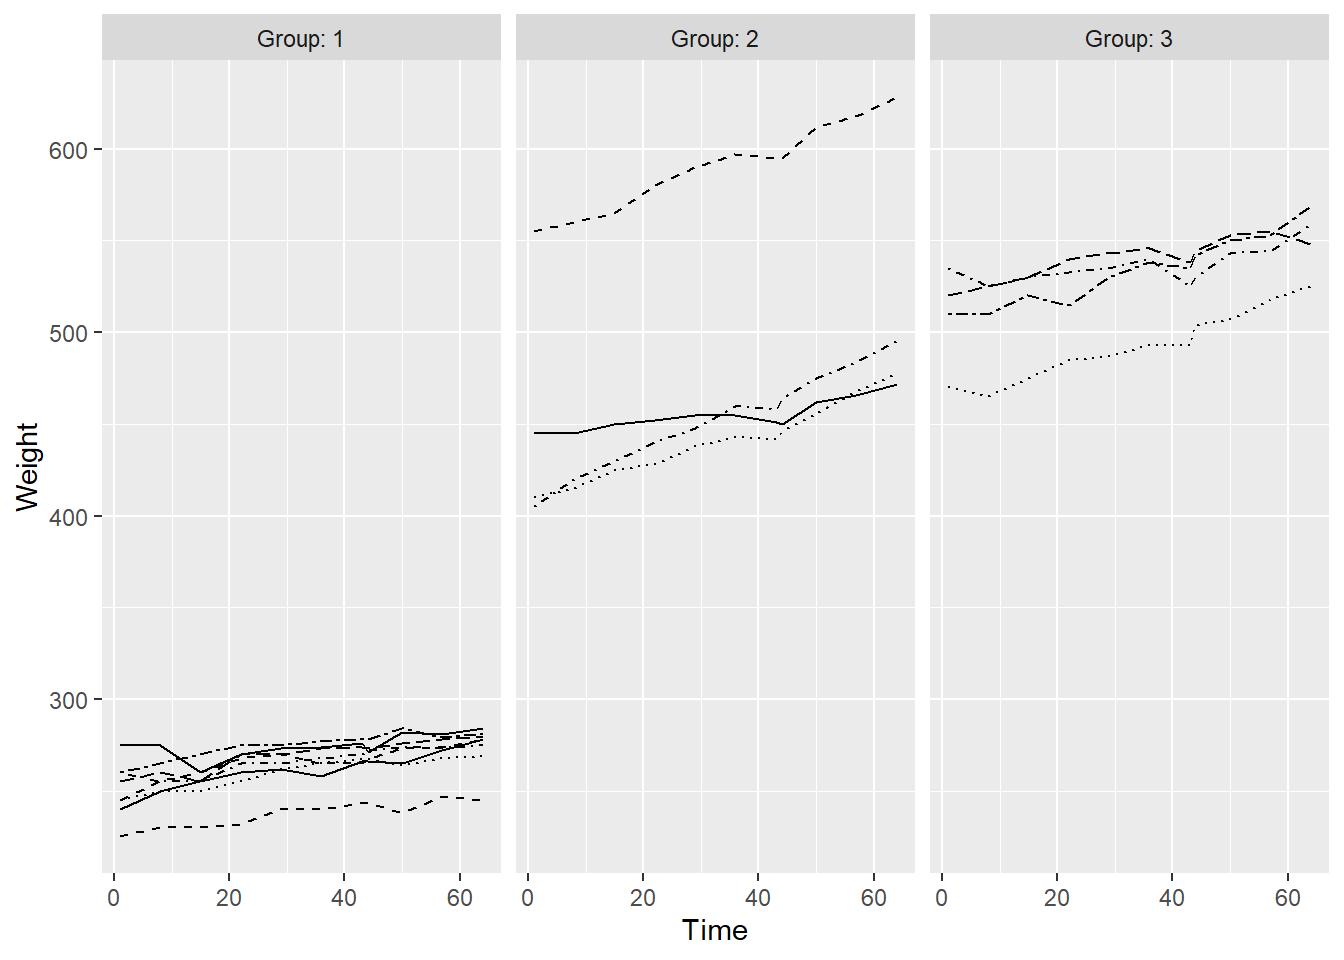
\includegraphics{chapter6_files/figure-latex/unnamed-chunk-2-1.pdf}

\begin{Shaded}
\begin{Highlighting}[]
\NormalTok{RATSL <-}\StringTok{ }\NormalTok{RATSL }\OperatorTok
\StringTok{  }\KeywordTok{group_by}\NormalTok{(Time) }\OperatorTok
\StringTok{  }\KeywordTok{mutate}\NormalTok{(}\DataTypeTok{stdWeight =}\NormalTok{ ((Weight }\OperatorTok{-}\StringTok{ }\KeywordTok{mean}\NormalTok{(Weight))}\OperatorTok{/}\KeywordTok{sd}\NormalTok{(Weight))) }\OperatorTok
\StringTok{  }\KeywordTok{ungroup}\NormalTok{()}
\end{Highlighting}
\end{Shaded}

\hypertarget{plot-again-with-the-standardised-bprs}{%
\section{Plot again with the standardised
bprs}\label{plot-again-with-the-standardised-bprs}}

\begin{Shaded}
\begin{Highlighting}[]
\KeywordTok{ggplot}\NormalTok{(RATSL, }\KeywordTok{aes}\NormalTok{(}\DataTypeTok{x =}\NormalTok{ Time, }\DataTypeTok{y =}\NormalTok{ stdWeight, }\DataTypeTok{linetype =}\NormalTok{ ID)) }\OperatorTok{+}
\StringTok{  }\KeywordTok{geom_line}\NormalTok{() }\OperatorTok{+}
\StringTok{  }\KeywordTok{scale_linetype_manual}\NormalTok{(}\DataTypeTok{values =} \KeywordTok{rep}\NormalTok{(}\DecValTok{1}\OperatorTok{:}\DecValTok{10}\NormalTok{, }\DataTypeTok{times=}\DecValTok{4}\NormalTok{)) }\OperatorTok{+}
\StringTok{  }\KeywordTok{facet_grid}\NormalTok{(. }\OperatorTok{~}\StringTok{ }\NormalTok{Group, }\DataTypeTok{labeller =}\NormalTok{ label_both) }\OperatorTok{+}
\StringTok{  }\KeywordTok{scale_y_continuous}\NormalTok{(}\DataTypeTok{name =} \StringTok{"standardized weight"}\NormalTok{)}
\end{Highlighting}
\end{Shaded}

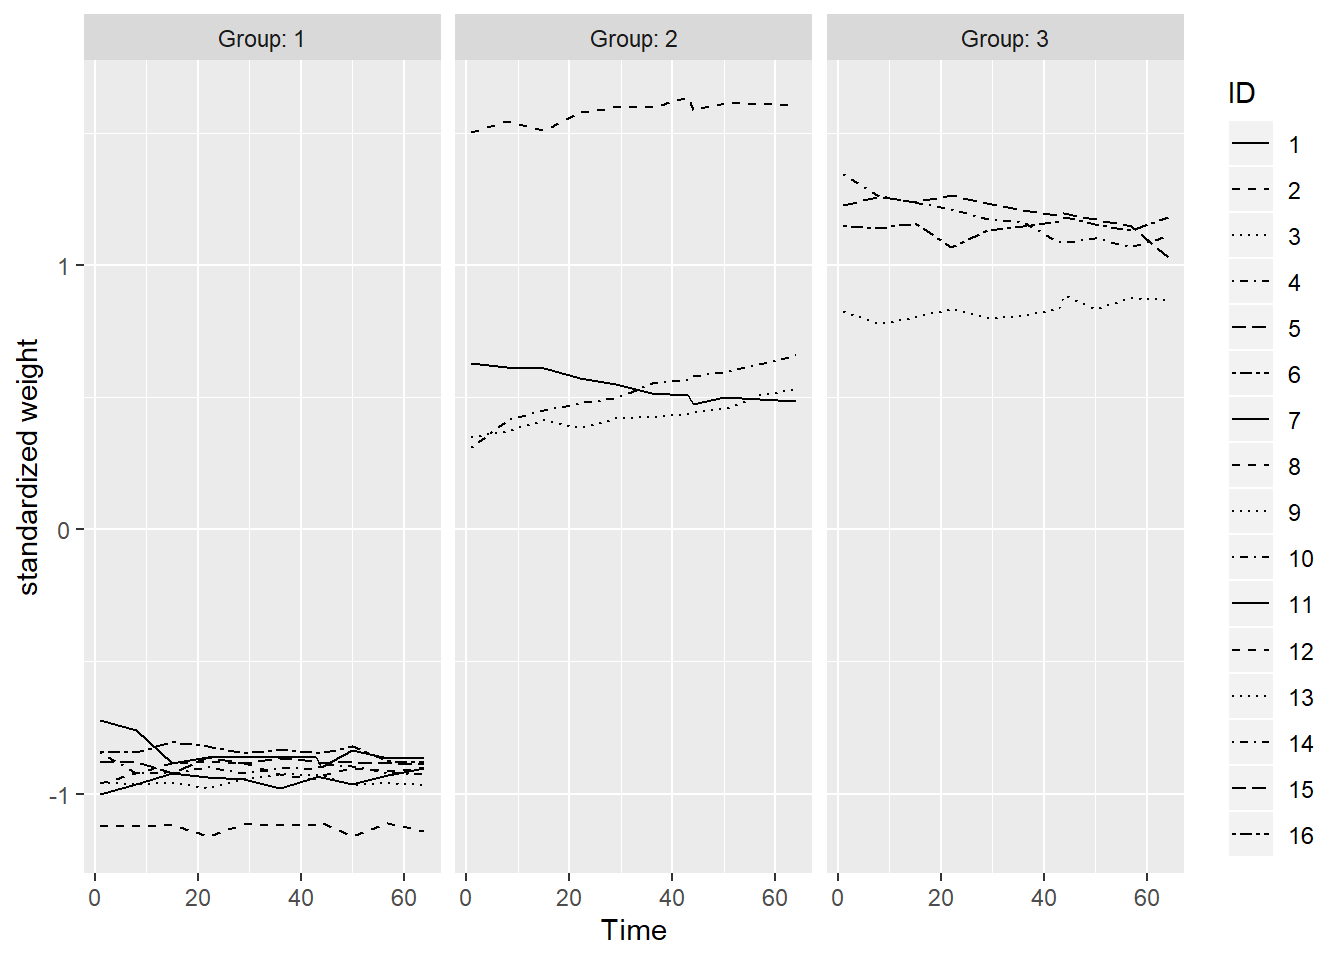
\includegraphics{chapter6_files/figure-latex/unnamed-chunk-4-1.pdf}

\begin{Shaded}
\begin{Highlighting}[]
\NormalTok{n <-}\StringTok{ }\NormalTok{RATSL}\OperatorTok{$}\NormalTok{Time }\OperatorTok\StringTok{ }\KeywordTok{unique}\NormalTok{() }\OperatorTok\StringTok{ }\KeywordTok{length}\NormalTok{()}


\CommentTok{# Summary data with mean and standard error of bprs by treatment and week }
\NormalTok{RATSS <-}\StringTok{ }\NormalTok{RATSL }\OperatorTok
\StringTok{  }\KeywordTok{group_by}\NormalTok{(Group, Time) }\OperatorTok
\StringTok{  }\KeywordTok{summarise}\NormalTok{( }\DataTypeTok{mean =} \KeywordTok{mean}\NormalTok{(Weight), }\DataTypeTok{se =} \KeywordTok{sd}\NormalTok{(Weight)}\OperatorTok{/}\KeywordTok{sqrt}\NormalTok{(n) ) }\OperatorTok
\StringTok{  }\KeywordTok{ungroup}\NormalTok{()}
\end{Highlighting}
\end{Shaded}

\begin{Shaded}
\begin{Highlighting}[]
\KeywordTok{ggplot}\NormalTok{(RATSS, }\KeywordTok{aes}\NormalTok{(}\DataTypeTok{x =}\NormalTok{ Time, }\DataTypeTok{y =}\NormalTok{ mean, }\DataTypeTok{linetype =}\NormalTok{ Group, }\DataTypeTok{shape =}\NormalTok{ Group)) }\OperatorTok{+}
\StringTok{  }\KeywordTok{geom_line}\NormalTok{() }\OperatorTok{+}
\StringTok{  }\KeywordTok{scale_linetype_manual}\NormalTok{(}\DataTypeTok{values =} \KeywordTok{c}\NormalTok{(}\DecValTok{1}\NormalTok{,}\DecValTok{2}\NormalTok{,}\DecValTok{3}\NormalTok{)) }\OperatorTok{+}
\StringTok{  }\KeywordTok{geom_point}\NormalTok{(}\DataTypeTok{size=}\DecValTok{3}\NormalTok{) }\OperatorTok{+}
\StringTok{  }\KeywordTok{scale_shape_manual}\NormalTok{(}\DataTypeTok{values =} \KeywordTok{c}\NormalTok{(}\DecValTok{1}\NormalTok{,}\DecValTok{2}\NormalTok{,}\DecValTok{3}\NormalTok{)) }\OperatorTok{+}
\StringTok{  }\KeywordTok{geom_errorbar}\NormalTok{(}\KeywordTok{aes}\NormalTok{(}\DataTypeTok{ymin=}\NormalTok{mean}\OperatorTok{-}\NormalTok{se, }\DataTypeTok{ymax=}\NormalTok{mean}\OperatorTok{+}\NormalTok{se, }\DataTypeTok{linetype=}\StringTok{"1"}\NormalTok{), }\DataTypeTok{width=}\FloatTok{0.3}\NormalTok{) }\OperatorTok{+}
\StringTok{  }\KeywordTok{theme}\NormalTok{(}\DataTypeTok{legend.position =} \KeywordTok{c}\NormalTok{(}\FloatTok{0.8}\NormalTok{,}\FloatTok{0.8}\NormalTok{)) }\OperatorTok{+}
\StringTok{  }\KeywordTok{scale_y_continuous}\NormalTok{(}\DataTypeTok{name =} \StringTok{"mean(Weight) +/- se(Weight)"}\NormalTok{)}
\end{Highlighting}
\end{Shaded}

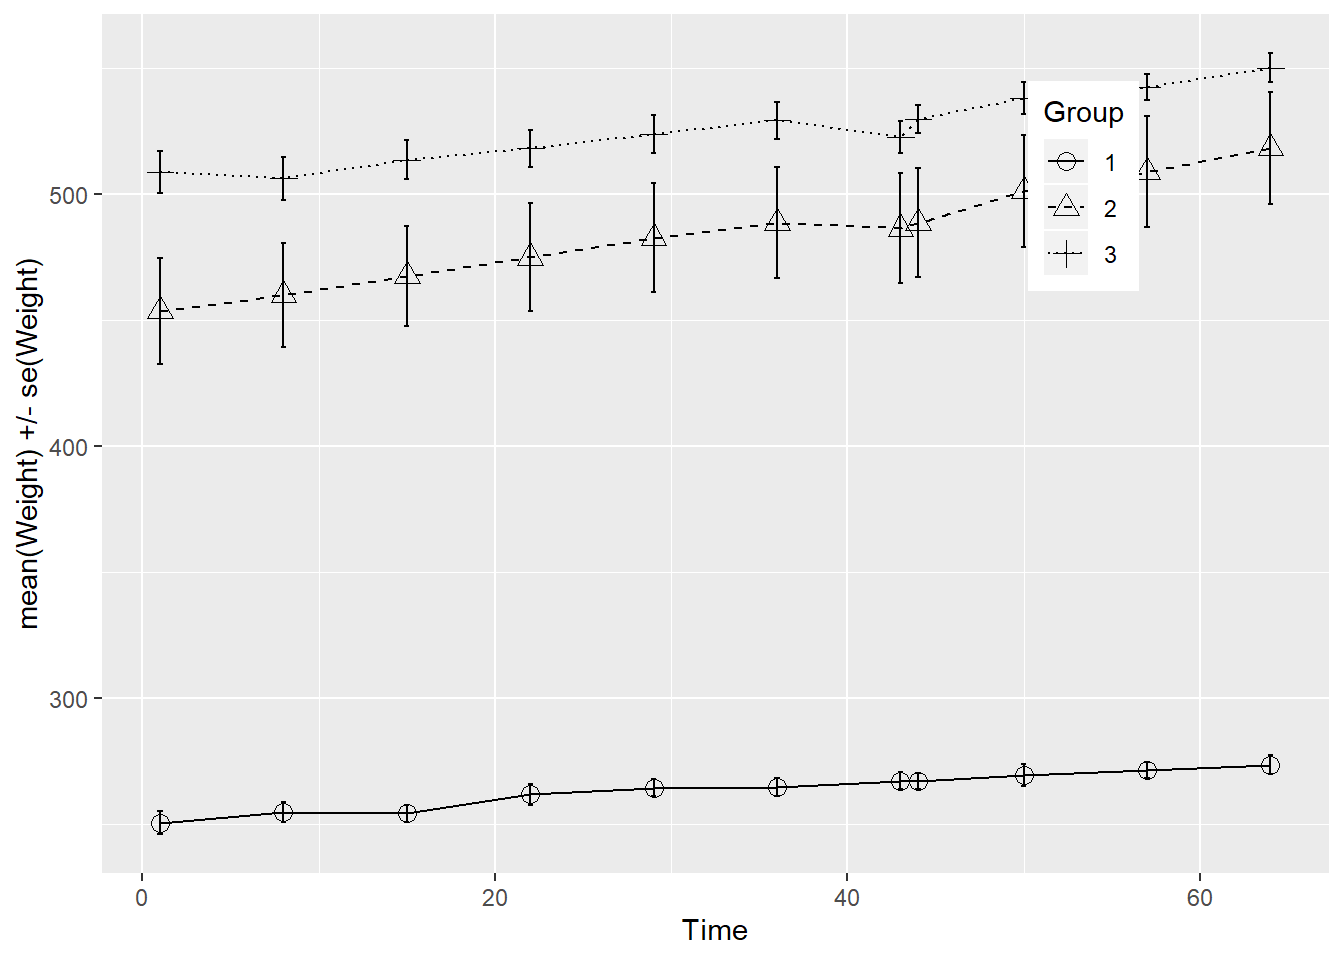
\includegraphics{chapter6_files/figure-latex/unnamed-chunk-6-1.pdf}

\begin{Shaded}
\begin{Highlighting}[]
\NormalTok{RATSL64S <-}\StringTok{ }\NormalTok{RATSL }\OperatorTok
\StringTok{  }\KeywordTok{filter}\NormalTok{(Time }\OperatorTok{>}\StringTok{ }\DecValTok{1}\NormalTok{) }\OperatorTok
\StringTok{  }\KeywordTok{group_by}\NormalTok{(Group, ID) }\OperatorTok
\StringTok{  }\KeywordTok{summarise}\NormalTok{(}\DataTypeTok{average=}\KeywordTok{mean}\NormalTok{(Weight)) }\OperatorTok
\StringTok{  }\KeywordTok{ungroup}\NormalTok{()}
\CommentTok{# Glimpse the data}
\KeywordTok{glimpse}\NormalTok{(RATSL64S)}
\end{Highlighting}
\end{Shaded}

\begin{verbatim}
## Observations: 16
## Variables: 3
## $ Group   <fct> 1, 1, 1, 1, 1, 1, 1, 1, 2, 2, 2, 2, 3, 3, 3, 3
## $ ID      <fct> 1, 2, 3, 4, 5, 6, 7, 8, 9, 10, 11, 12, 13, 14, 15, 16
## $ average <dbl> 263.2, 238.9, 261.7, 267.2, 270.9, 276.2, 274.6, 267.5...
\end{verbatim}

\begin{Shaded}
\begin{Highlighting}[]
\CommentTok{# Draw a boxplot of the mean versus treatment}
\KeywordTok{ggplot}\NormalTok{(RATSL64S, }\KeywordTok{aes}\NormalTok{(}\DataTypeTok{x =}\NormalTok{ Group, }\DataTypeTok{y =}\NormalTok{ average)) }\OperatorTok{+}
\StringTok{  }\KeywordTok{geom_boxplot}\NormalTok{() }\OperatorTok{+}
\StringTok{  }\KeywordTok{stat_summary}\NormalTok{(}\DataTypeTok{fun.y =} \StringTok{"mean"}\NormalTok{, }\DataTypeTok{geom =} \StringTok{"point"}\NormalTok{, }\DataTypeTok{shape=}\DecValTok{23}\NormalTok{, }\DataTypeTok{size=}\DecValTok{4}\NormalTok{, }\DataTypeTok{fill =} \StringTok{"white"}\NormalTok{) }\OperatorTok{+}
\StringTok{  }\KeywordTok{scale_y_continuous}\NormalTok{(}\DataTypeTok{name =} \StringTok{"mean(Weight), periods 8-64"}\NormalTok{)}
\end{Highlighting}
\end{Shaded}

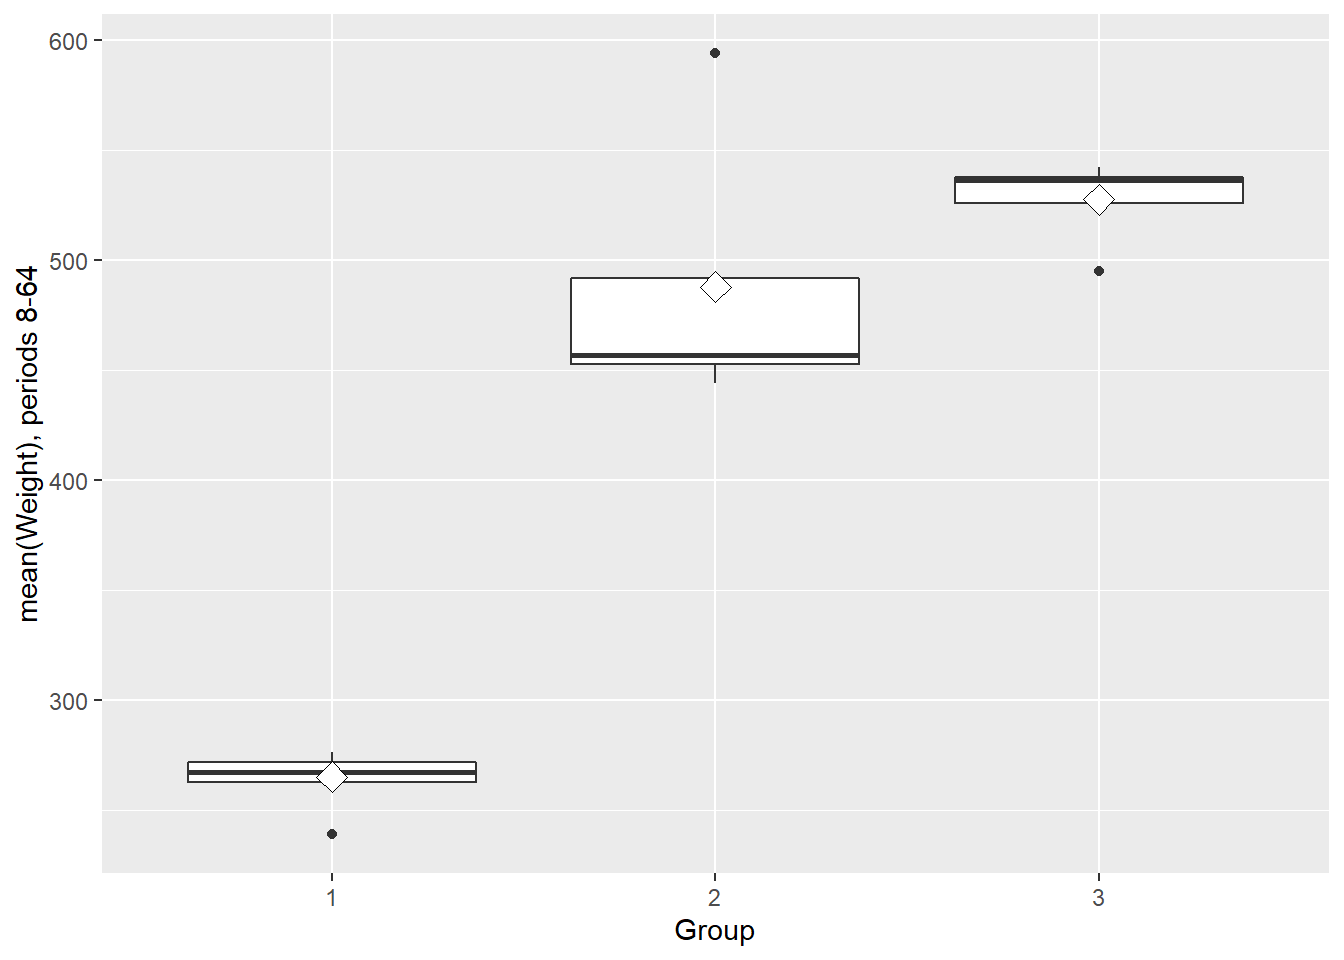
\includegraphics{chapter6_files/figure-latex/unnamed-chunk-8-1.pdf}

\begin{Shaded}
\begin{Highlighting}[]
\NormalTok{RATSL64SF <-}\StringTok{ }\NormalTok{RATSL64S }\OperatorTok\StringTok{ }\KeywordTok{filter}\NormalTok{(average }\OperatorTok{<}\StringTok{ }\DecValTok{580}\NormalTok{, average }\OperatorTok{>}\StringTok{ }\DecValTok{240}\NormalTok{, average }\OperatorTok{!=}\StringTok{ }\FloatTok{495.2}\NormalTok{)}
\KeywordTok{ggplot}\NormalTok{(RATSL64SF, }\KeywordTok{aes}\NormalTok{(}\DataTypeTok{x =}\NormalTok{ Group, }\DataTypeTok{y =}\NormalTok{ average)) }\OperatorTok{+}
\StringTok{  }\KeywordTok{geom_boxplot}\NormalTok{() }\OperatorTok{+}
\StringTok{  }\KeywordTok{stat_summary}\NormalTok{(}\DataTypeTok{fun.y =} \StringTok{"mean"}\NormalTok{, }\DataTypeTok{geom =} \StringTok{"point"}\NormalTok{, }\DataTypeTok{shape=}\DecValTok{23}\NormalTok{, }\DataTypeTok{size=}\DecValTok{4}\NormalTok{, }\DataTypeTok{fill =} \StringTok{"white"}\NormalTok{) }\OperatorTok{+}
\StringTok{  }\KeywordTok{scale_y_continuous}\NormalTok{(}\DataTypeTok{name =} \StringTok{"mean(Weight), periods 8-64"}\NormalTok{)}
\end{Highlighting}
\end{Shaded}

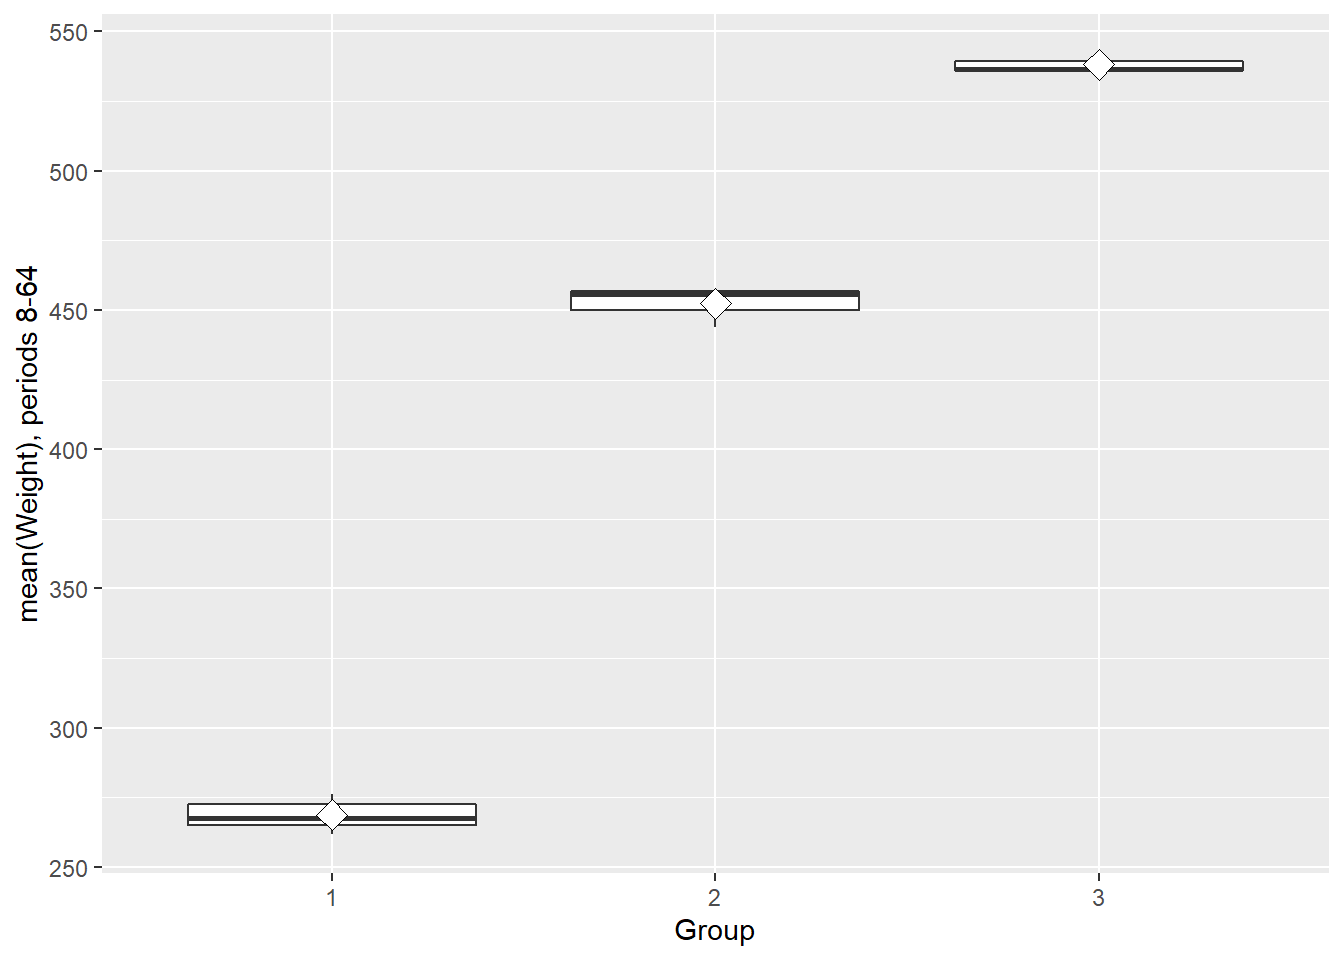
\includegraphics{chapter6_files/figure-latex/unnamed-chunk-9-1.pdf}

\begin{Shaded}
\begin{Highlighting}[]
\NormalTok{RATSL8S2 <-}\StringTok{ }\NormalTok{RATSL64S }\OperatorTok
\StringTok{  }\KeywordTok{mutate}\NormalTok{(}\DataTypeTok{baseline =}\NormalTok{ RATS}\OperatorTok{$}\NormalTok{WD1)}
\end{Highlighting}
\end{Shaded}

\begin{Shaded}
\begin{Highlighting}[]
\NormalTok{fit <-}\StringTok{ }\KeywordTok{lm}\NormalTok{(average }\OperatorTok{~}\StringTok{ }\NormalTok{baseline }\OperatorTok{+}\StringTok{ }\NormalTok{Group, }\DataTypeTok{data =}\NormalTok{ RATSL8S2)}
\CommentTok{# Compute the analysis of variance table for the fitted model with anova()}
\KeywordTok{anova}\NormalTok{(fit)}
\end{Highlighting}
\end{Shaded}

\begin{verbatim}
## Analysis of Variance Table
## 
## Response: average
##           Df Sum Sq Mean Sq   F value   Pr(>F)    
## baseline   1 253625  253625 1859.8201 1.57e-14 ***
## Group      2    879     439    3.2219  0.07586 .  
## Residuals 12   1636     136                       
## ---
## Signif. codes:  0 '***' 0.001 '**' 0.01 '*' 0.05 '.' 0.1 ' ' 1
\end{verbatim}

The data has 360 observations and 5 variables. The variables describe
the sum of the scale measures levels, what treatment group the
individual is assigned, and when the measures were collected.

\begin{Shaded}
\begin{Highlighting}[]
\KeywordTok{summary}\NormalTok{(BPRSL}\OperatorTok{$}\NormalTok{bprs)}
\end{Highlighting}
\end{Shaded}

\begin{verbatim}
##    Min. 1st Qu.  Median    Mean 3rd Qu.    Max. 
##   18.00   27.00   35.00   37.66   43.00   95.00
\end{verbatim}

\begin{Shaded}
\begin{Highlighting}[]
\KeywordTok{summary}\NormalTok{(BPRSL}\OperatorTok{$}\NormalTok{treatment)}
\end{Highlighting}
\end{Shaded}

\begin{verbatim}
##    Min. 1st Qu.  Median    Mean 3rd Qu.    Max. 
##     1.0     1.0     1.5     1.5     2.0     2.0
\end{verbatim}

\begin{Shaded}
\begin{Highlighting}[]
\NormalTok{BPRSL}\OperatorTok{$}\NormalTok{treatment <-}\StringTok{ }\KeywordTok{factor}\NormalTok{(BPRSL}\OperatorTok{$}\NormalTok{treatment)}
\end{Highlighting}
\end{Shaded}

The median of bprs rating is 35 and mean is 37.66. Some individuals
diviate from this average signficantly, since the minimum of the rating
is 18 and maximum 95.

\begin{Shaded}
\begin{Highlighting}[]
\NormalTok{BPRSL}\OperatorTok{$}\NormalTok{subject <-}\StringTok{ }\KeywordTok{factor}\NormalTok{(BPRSL}\OperatorTok{$}\NormalTok{subject)}
\NormalTok{BPRSL}\OperatorTok{$}\NormalTok{group <-}\StringTok{ }\KeywordTok{factor}\NormalTok{(BPRSL}\OperatorTok{$}\NormalTok{treatment)}
\KeywordTok{ggplot}\NormalTok{(BPRSL, }\KeywordTok{aes}\NormalTok{(}\DataTypeTok{x =}\NormalTok{ week, }\DataTypeTok{y=}\NormalTok{ bprs, }\DataTypeTok{linetype =}\NormalTok{ subject, }\DataTypeTok{col =}\NormalTok{ treatment)) }\OperatorTok{+}
\StringTok{  }\KeywordTok{geom_line}\NormalTok{() }\OperatorTok{+}
\StringTok{   }\KeywordTok{scale_linetype_manual}\NormalTok{(}\DataTypeTok{values =} \KeywordTok{rep}\NormalTok{(}\DecValTok{1}\OperatorTok{:}\DecValTok{10}\NormalTok{, }\DataTypeTok{times=}\DecValTok{4}\NormalTok{)) }\OperatorTok{+}
\StringTok{ }
\StringTok{    }\KeywordTok{theme}\NormalTok{(}\DataTypeTok{legend.position =} \StringTok{"none"}\NormalTok{) }\OperatorTok{+}
\StringTok{    }\KeywordTok{scale_y_continuous}\NormalTok{(}\DataTypeTok{limits =} \KeywordTok{c}\NormalTok{(}\KeywordTok{min}\NormalTok{(BPRSL}\OperatorTok{$}\NormalTok{bprs), }\KeywordTok{max}\NormalTok{(BPRSL}\OperatorTok{$}\NormalTok{bprs)))}
\end{Highlighting}
\end{Shaded}

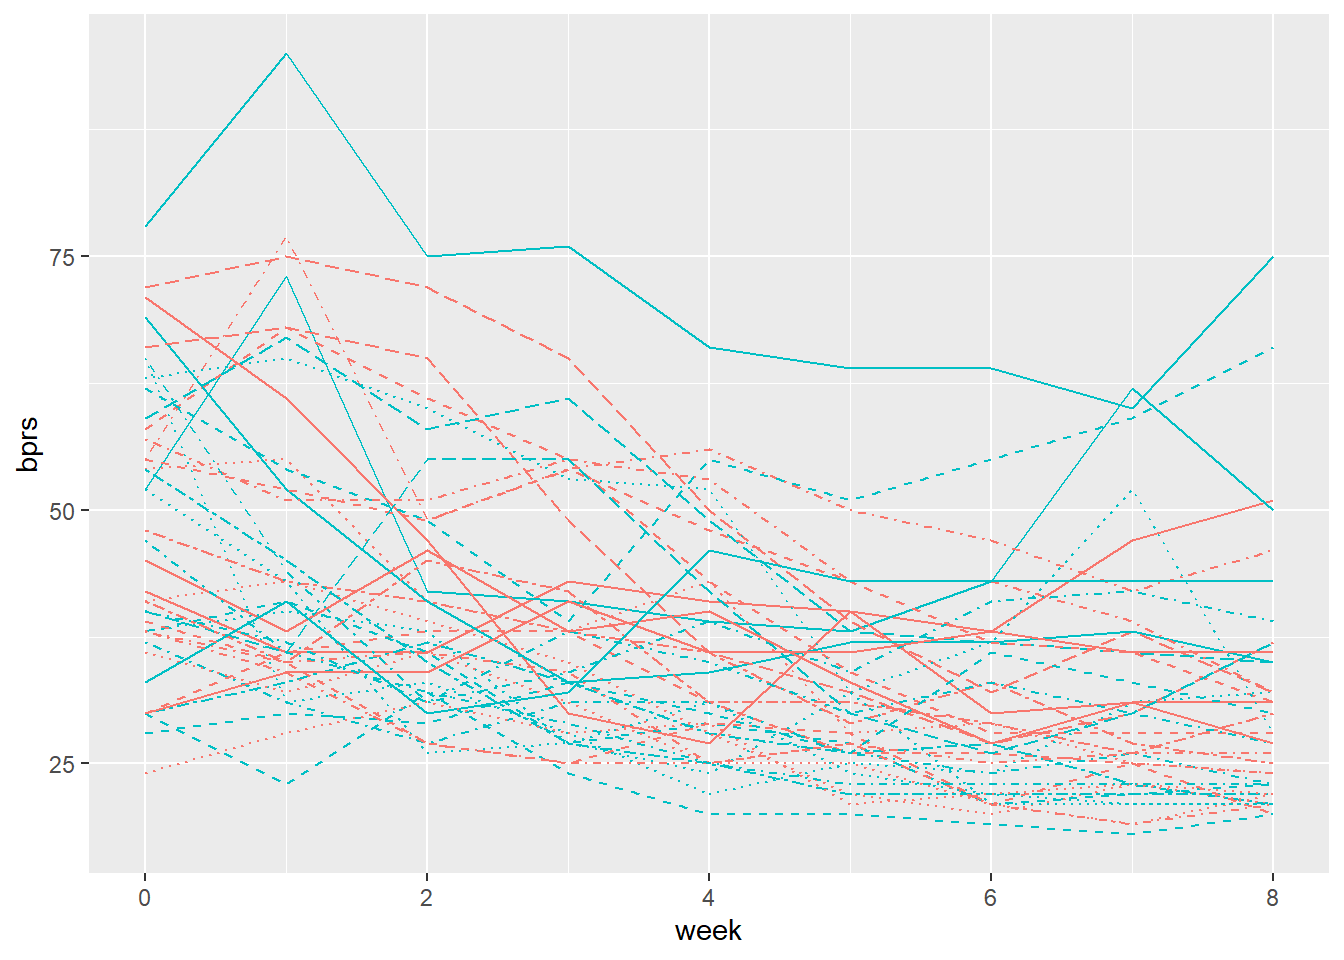
\includegraphics{chapter6_files/figure-latex/unnamed-chunk-13-1.pdf}

In the blue are people who received treatment 2, and in red people
received treatment 1. Maybe we get a clearer picture, if we plot these
two groups individually by group:

\begin{Shaded}
\begin{Highlighting}[]
\NormalTok{BPRSL}\OperatorTok{$}\NormalTok{subject <-}\StringTok{ }\KeywordTok{factor}\NormalTok{(BPRSL}\OperatorTok{$}\NormalTok{subject)}
\NormalTok{BPRSL}\OperatorTok{$}\NormalTok{group <-}\StringTok{ }\KeywordTok{factor}\NormalTok{(BPRSL}\OperatorTok{$}\NormalTok{treatment)}
\KeywordTok{ggplot}\NormalTok{(BPRSL, }\KeywordTok{aes}\NormalTok{(}\DataTypeTok{x =}\NormalTok{ week, }\DataTypeTok{y=}\NormalTok{ bprs, }\DataTypeTok{linetype =}\NormalTok{ subject, }\DataTypeTok{col =}\NormalTok{ treatment)) }\OperatorTok{+}
\StringTok{  }\KeywordTok{geom_line}\NormalTok{() }\OperatorTok{+}
\StringTok{   }\KeywordTok{scale_linetype_manual}\NormalTok{(}\DataTypeTok{values =} \KeywordTok{rep}\NormalTok{(}\DecValTok{1}\OperatorTok{:}\DecValTok{10}\NormalTok{, }\DataTypeTok{times=}\DecValTok{4}\NormalTok{)) }\OperatorTok{+}
\StringTok{      }\KeywordTok{facet_grid}\NormalTok{(. }\OperatorTok{~}\StringTok{ }\NormalTok{treatment, }\DataTypeTok{labeller =}\NormalTok{ label_both) }\OperatorTok{+}
\StringTok{      }\KeywordTok{theme}\NormalTok{(}\DataTypeTok{legend.position =} \StringTok{"none"}\NormalTok{) }\OperatorTok{+}
\StringTok{    }\KeywordTok{scale_y_continuous}\NormalTok{(}\DataTypeTok{limits =} \KeywordTok{c}\NormalTok{(}\KeywordTok{min}\NormalTok{(BPRSL}\OperatorTok{$}\NormalTok{bprs), }\KeywordTok{max}\NormalTok{(BPRSL}\OperatorTok{$}\NormalTok{bprs)))}
\end{Highlighting}
\end{Shaded}

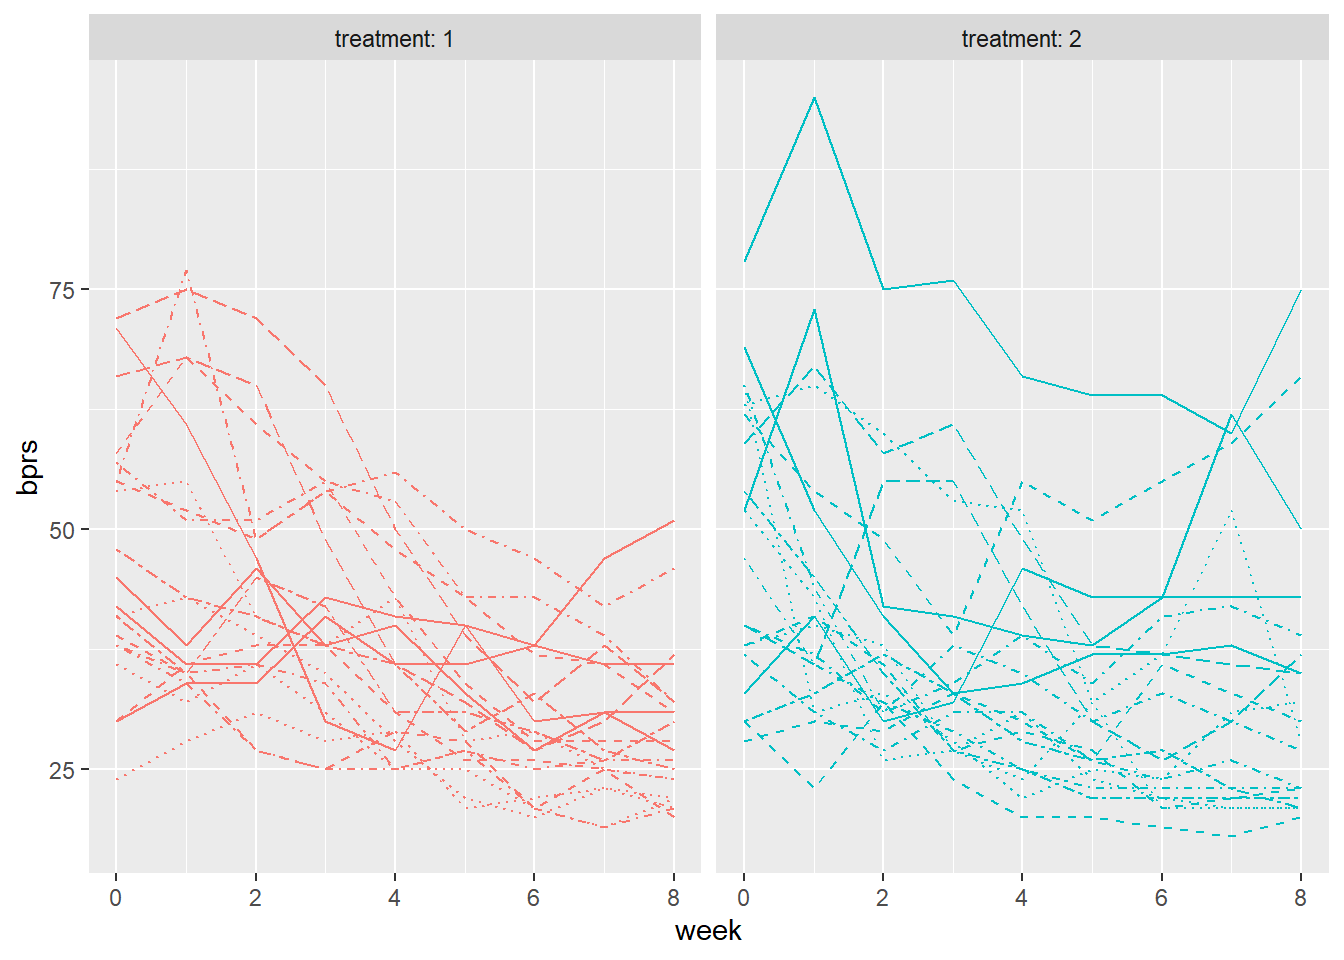
\includegraphics{chapter6_files/figure-latex/unnamed-chunk-14-1.pdf}

It may be difficult to distinguish a clear trend from these plots. For
some people, it seems that treatment in group 1 or group 2 decreased
BRPS points, but for some the treatment period did not.

\begin{Shaded}
\begin{Highlighting}[]
\CommentTok{# create a regression model}
\NormalTok{BPRSL_reg <-}\StringTok{ }\KeywordTok{lm}\NormalTok{(bprs }\OperatorTok{~}\StringTok{ }\NormalTok{week }\OperatorTok{+}\StringTok{ }\NormalTok{treatment, }\DataTypeTok{data =}\NormalTok{ BPRSL)}
\CommentTok{# print out a summary of the model}
\KeywordTok{summary}\NormalTok{(BPRSL_reg)}
\end{Highlighting}
\end{Shaded}

\begin{verbatim}
## 
## Call:
## lm(formula = bprs ~ week + treatment, data = BPRSL)
## 
## Residuals:
##     Min      1Q  Median      3Q     Max 
## -22.454  -8.965  -3.196   7.002  50.244 
## 
## Coefficients:
##             Estimate Std. Error t value Pr(>|t|)    
## (Intercept)  46.4539     1.3670  33.982   <2e-16 ***
## week         -2.2704     0.2524  -8.995   <2e-16 ***
## treatment2    0.5722     1.3034   0.439    0.661    
## ---
## Signif. codes:  0 '***' 0.001 '**' 0.01 '*' 0.05 '.' 0.1 ' ' 1
## 
## Residual standard error: 12.37 on 357 degrees of freedom
## Multiple R-squared:  0.1851, Adjusted R-squared:  0.1806 
## F-statistic: 40.55 on 2 and 357 DF,  p-value: < 2.2e-16
\end{verbatim}

From a simple regression model bprs = week + treatment, we see that the
p-value for treatment2 is 0.661. Therefore, we cannot reject the null
hypothesis that the coefficient of treatment2 is zero. Here we assume
unrealistically indepence to the repeated measures of bprs for
individuals.

\begin{Shaded}
\begin{Highlighting}[]
\CommentTok{# access library lme4}
\KeywordTok{library}\NormalTok{(lme4)}
\end{Highlighting}
\end{Shaded}

\begin{verbatim}
## Loading required package: Matrix
\end{verbatim}

\begin{verbatim}
## 
## Attaching package: 'Matrix'
\end{verbatim}

\begin{verbatim}
## The following objects are masked from 'package:tidyr':
## 
##     expand, pack, unpack
\end{verbatim}

\begin{Shaded}
\begin{Highlighting}[]
\CommentTok{# Fitting a random intercept model allows the linear regression fit for each rat to differ # in intercept from other rats.}
\CommentTok{# Create a random intercept model}
\NormalTok{BPRSL_ref <-}\StringTok{ }\KeywordTok{lmer}\NormalTok{(bprs }\OperatorTok{~}\StringTok{ }\NormalTok{week }\OperatorTok{+}\StringTok{ }\NormalTok{treatment }\OperatorTok{+}\StringTok{ }\NormalTok{(}\DecValTok{1} \OperatorTok{|}\StringTok{ }\NormalTok{subject), }\DataTypeTok{data =}\NormalTok{ BPRSL, }\DataTypeTok{REML =} \OtherTok{FALSE}\NormalTok{)}
\CommentTok{# Print the summary of the model}
\KeywordTok{summary}\NormalTok{(BPRSL_ref)}
\end{Highlighting}
\end{Shaded}

\begin{verbatim}
## Linear mixed model fit by maximum likelihood  ['lmerMod']
## Formula: bprs ~ week + treatment + (1 | subject)
##    Data: BPRSL
## 
##      AIC      BIC   logLik deviance df.resid 
##   2748.7   2768.1  -1369.4   2738.7      355 
## 
## Scaled residuals: 
##     Min      1Q  Median      3Q     Max 
## -3.0481 -0.6749 -0.1361  0.4813  3.4855 
## 
## Random effects:
##  Groups   Name        Variance Std.Dev.
##  subject  (Intercept)  47.41    6.885  
##  Residual             104.21   10.208  
## Number of obs: 360, groups:  subject, 20
## 
## Fixed effects:
##             Estimate Std. Error t value
## (Intercept)  46.4539     1.9090  24.334
## week         -2.2704     0.2084 -10.896
## treatment2    0.5722     1.0761   0.532
## 
## Correlation of Fixed Effects:
##            (Intr) week  
## week       -0.437       
## treatment2 -0.282  0.000
\end{verbatim}

With the above random intercept model, we can allow individual BPRS to
differ with an intercept term, that is usually not the same as for other
individuals. Here, the standard errors are lower than in the simple
linear regression model. The conclusion does not change in this model.

\begin{Shaded}
\begin{Highlighting}[]
\CommentTok{# create a random intercept and random slope model}
\NormalTok{BPRSL_ref1 <-}\StringTok{ }\KeywordTok{lmer}\NormalTok{(bprs }\OperatorTok{~}\StringTok{ }\NormalTok{week }\OperatorTok{+}\StringTok{ }\NormalTok{treatment }\OperatorTok{+}\StringTok{ }\NormalTok{(week }\OperatorTok{|}\StringTok{ }\NormalTok{subject), }\DataTypeTok{data =}\NormalTok{ BPRSL, }\DataTypeTok{REML =} \OtherTok{FALSE}\NormalTok{)}
\CommentTok{# Fitting a random intercept and random slope model allows the linear regression fits for each individual to differ in intercept but also in slope. This way it is possible to account for the individual differences in the rats' growth profiles, but also the   effect of time.}
\CommentTok{# print a summary of the model}
\KeywordTok{summary}\NormalTok{(BPRSL_ref1)}
\end{Highlighting}
\end{Shaded}

\begin{verbatim}
## Linear mixed model fit by maximum likelihood  ['lmerMod']
## Formula: bprs ~ week + treatment + (week | subject)
##    Data: BPRSL
## 
##      AIC      BIC   logLik deviance df.resid 
##   2745.4   2772.6  -1365.7   2731.4      353 
## 
## Scaled residuals: 
##     Min      1Q  Median      3Q     Max 
## -2.8919 -0.6194 -0.0691  0.5531  3.7977 
## 
## Random effects:
##  Groups   Name        Variance Std.Dev. Corr 
##  subject  (Intercept) 64.8222  8.0512        
##           week         0.9609  0.9803   -0.51
##  Residual             97.4304  9.8707        
## Number of obs: 360, groups:  subject, 20
## 
## Fixed effects:
##             Estimate Std. Error t value
## (Intercept)  46.4539     2.1052  22.066
## week         -2.2704     0.2977  -7.626
## treatment2    0.5722     1.0405   0.550
## 
## Correlation of Fixed Effects:
##            (Intr) week  
## week       -0.582       
## treatment2 -0.247  0.000
\end{verbatim}

\begin{Shaded}
\begin{Highlighting}[]
\CommentTok{# perform an ANOVA test on the two models}
\KeywordTok{anova}\NormalTok{(BPRSL_ref1, BPRSL_ref)}
\end{Highlighting}
\end{Shaded}

\begin{verbatim}
## Data: BPRSL
## Models:
## BPRSL_ref: bprs ~ week + treatment + (1 | subject)
## BPRSL_ref1: bprs ~ week + treatment + (week | subject)
##            Df    AIC    BIC  logLik deviance  Chisq Chi Df Pr(>Chisq)  
## BPRSL_ref   5 2748.7 2768.1 -1369.4   2738.7                           
## BPRSL_ref1  7 2745.4 2772.6 -1365.7   2731.4 7.2721      2    0.02636 *
## ---
## Signif. codes:  0 '***' 0.001 '**' 0.01 '*' 0.05 '.' 0.1 ' ' 1
\end{verbatim}

Fitting the random intercept and slope model to the BPRS data results
compared to the the fixed effects model are very similar. However, the
chi-squared statistics and p-value of the likelihood ratio test between
BPRSL\_ref and BPRS\_ref1 are very low, indicating that the fit is
better in BPRS\_ref1, that is compared to BPRS\_ref model.

\begin{Shaded}
\begin{Highlighting}[]
\CommentTok{# create a random intercept and random slope model}
\CommentTok{# Add a interaction term}
\NormalTok{BPRSL_ref2 <-}\StringTok{ }\KeywordTok{lmer}\NormalTok{(bprs }\OperatorTok{~}\StringTok{ }\NormalTok{week }\OperatorTok{*}\StringTok{ }\NormalTok{treatment }\OperatorTok{+}\StringTok{ }\NormalTok{(week }\OperatorTok{|}\StringTok{ }\NormalTok{subject), }\DataTypeTok{data =}\NormalTok{ BPRSL, }\DataTypeTok{REML =} \OtherTok{FALSE}\NormalTok{)}
\CommentTok{# print a summary of the model}
\KeywordTok{summary}\NormalTok{(BPRSL_ref2)}
\end{Highlighting}
\end{Shaded}

\begin{verbatim}
## Linear mixed model fit by maximum likelihood  ['lmerMod']
## Formula: bprs ~ week * treatment + (week | subject)
##    Data: BPRSL
## 
##      AIC      BIC   logLik deviance df.resid 
##   2744.3   2775.4  -1364.1   2728.3      352 
## 
## Scaled residuals: 
##     Min      1Q  Median      3Q     Max 
## -3.0512 -0.6271 -0.0768  0.5288  3.9260 
## 
## Random effects:
##  Groups   Name        Variance Std.Dev. Corr 
##  subject  (Intercept) 64.9964  8.0620        
##           week         0.9687  0.9842   -0.51
##  Residual             96.4707  9.8220        
## Number of obs: 360, groups:  subject, 20
## 
## Fixed effects:
##                 Estimate Std. Error t value
## (Intercept)      47.8856     2.2521  21.262
## week             -2.6283     0.3589  -7.323
## treatment2       -2.2911     1.9090  -1.200
## week:treatment2   0.7158     0.4010   1.785
## 
## Correlation of Fixed Effects:
##             (Intr) week   trtmn2
## week        -0.650              
## treatment2  -0.424  0.469       
## wek:trtmnt2  0.356 -0.559 -0.840
\end{verbatim}

\begin{Shaded}
\begin{Highlighting}[]
\CommentTok{# perform an ANOVA test on the two models}
\KeywordTok{anova}\NormalTok{(BPRSL_ref2, BPRSL_ref1)}
\end{Highlighting}
\end{Shaded}

\begin{verbatim}
## Data: BPRSL
## Models:
## BPRSL_ref1: bprs ~ week + treatment + (week | subject)
## BPRSL_ref2: bprs ~ week * treatment + (week | subject)
##            Df    AIC    BIC  logLik deviance  Chisq Chi Df Pr(>Chisq)  
## BPRSL_ref1  7 2745.4 2772.6 -1365.7   2731.4                           
## BPRSL_ref2  8 2744.3 2775.4 -1364.1   2728.3 3.1712      1    0.07495 .
## ---
## Signif. codes:  0 '***' 0.001 '**' 0.01 '*' 0.05 '.' 0.1 ' ' 1
\end{verbatim}

Here, I created a random intercept and random slope model with an
interaction term of week and treatment, measuring how these terms affect
together bprs value.

The chi-squared statistics is low (3.17). P-value of the likelihood
ratio test between BPRSL\_ref1 and BPRS\_ref2 is 0.07495, indicating
that on 10 \% significance level, the model increases fit. However, on 5
\% significance level, we cannot make this conclusion.

\begin{Shaded}
\begin{Highlighting}[]
\CommentTok{# Create a vector of the fitted values}
\NormalTok{Fitted <-}\StringTok{ }\KeywordTok{fitted}\NormalTok{(BPRSL_ref2)}
\CommentTok{# Create a new column fitted to BPRSL}
\NormalTok{BPRSL <-}\StringTok{ }\NormalTok{BPRSL }\OperatorTok
\StringTok{  }\KeywordTok{mutate}\NormalTok{(Fitted)}
\KeywordTok{ggplot}\NormalTok{(BPRSL, }\KeywordTok{aes}\NormalTok{(}\DataTypeTok{x =}\NormalTok{ week, }\DataTypeTok{y=}\NormalTok{ Fitted, }\DataTypeTok{linetype =}\NormalTok{ subject, }\DataTypeTok{col =}\NormalTok{ treatment)) }\OperatorTok{+}
\StringTok{  }\KeywordTok{geom_line}\NormalTok{() }\OperatorTok{+}
\StringTok{   }\KeywordTok{scale_linetype_manual}\NormalTok{(}\DataTypeTok{values =} \KeywordTok{rep}\NormalTok{(}\DecValTok{1}\OperatorTok{:}\DecValTok{10}\NormalTok{, }\DataTypeTok{times=}\DecValTok{4}\NormalTok{)) }\OperatorTok{+}
\StringTok{      }\KeywordTok{facet_grid}\NormalTok{(. }\OperatorTok{~}\StringTok{ }\NormalTok{treatment, }\DataTypeTok{labeller =}\NormalTok{ label_both) }\OperatorTok{+}
\StringTok{      }\KeywordTok{theme}\NormalTok{(}\DataTypeTok{legend.position =} \StringTok{"none"}\NormalTok{) }\OperatorTok{+}
\StringTok{    }\KeywordTok{scale_y_continuous}\NormalTok{(}\DataTypeTok{limits =} \KeywordTok{c}\NormalTok{(}\KeywordTok{min}\NormalTok{(BPRSL}\OperatorTok{$}\NormalTok{Fitted), }\KeywordTok{max}\NormalTok{(BPRSL}\OperatorTok{$}\NormalTok{Fitted)))}
\end{Highlighting}
\end{Shaded}

\includegraphics{chapter6_files/figure-latex/unnamed-chunk-19-1.pdf}


\end{document}
